% Generated from ../paper_draft.md; see README.md for regeneration.
\documentclass[10pt,twocolumn,letterpaper]{article}
\usepackage[T1]{fontenc}
\usepackage[utf8]{inputenc}
\usepackage{newtxtext}
\usepackage[letterpaper,left=0.75in,right=0.75in,top=0.75in,bottom=0.8in,columnsep=0.25in]{geometry}
\usepackage{graphicx}
\usepackage{booktabs}
\usepackage{microtype}
\usepackage{caption}
\usepackage{titlesec}
\usepackage{xurl}
\usepackage[hidelinks]{hyperref}
\usepackage{flushend}
\graphicspath{{figures/}}
\hypersetup{pdftitle={Task Authorization, Export Guards and Bounded Recovery at the MCP Boundary},pdfauthor={Yannis ANDRE}}
\setlength{\parindent}{1em}
\setlength{\parskip}{0pt}
\setlength{\textfloatsep}{12pt plus 2pt minus 2pt}
\setlength{\dbltextfloatsep}{13pt plus 2pt minus 2pt}
\setlength{\floatsep}{10pt plus 2pt minus 2pt}
\renewcommand{\topfraction}{0.95}
\renewcommand{\dbltopfraction}{0.95}
\renewcommand{\textfraction}{0.05}
\renewcommand{\floatpagefraction}{0.8}
\renewcommand{\dblfloatpagefraction}{0.8}
\setcounter{topnumber}{3}
\setcounter{dbltopnumber}{1}
\setcounter{totalnumber}{5}
\captionsetup{font=small,labelfont=bf,skip=5pt}
\titleformat{\section}{\large\bfseries}{\thesection}{0.65em}{}
\titlespacing*{\section}{0pt}{9pt plus 2pt minus 1pt}{4pt}
\urlstyle{same}
\emergencystretch=1.2em
\clubpenalty=10000
\widowpenalty=10000
\pagestyle{plain}
\raggedbottom
\begin{document}

% Manuscript SHA-256: 7479525ac93d4f256d585e732772d19dc00653b5c4f239cf3073a79c15f6ac17
\twocolumn[{
\begin{center}
{\LARGE\bfseries Task Authorization, Export Guards and Bounded Recovery at the MCP Boundary\par}
\vspace{9pt}
\textbf{Yannis ANDRE}\par
\vspace{4pt}
{\small Computer Security and Digital Forensics Laboratory, Faculty of Computer Science, Goce Delcev University\par}
\vspace{5pt}
{\small Conducted in collaboration with and under the supervision of \textbf{Aleksandra Mileva} and \textbf{Aleksandar Velinov}.\par}
\end{center}
\noindent\begin{minipage}{\textwidth}\footnotesize \textbf{AI assistance disclosure.} Generative AI (OpenAI Codex) was used to refine the manuscript's wording and structure and to assist with prototype architecture, code implementation, tests, and experiment-analysis scripts. These uses are distinct from the actor and judge models evaluated in the experiments.\end{minipage}
\vspace{12pt}
}]
\section*{Abstract}
Tool-using agents may read confidential information for an internal check while being authorized to publish only a public summary. Account permissions and an allowed destination do not establish that the exported content respects that distinction. We implement an explicitly configured MCP proxy, an API-driven Python agent, an honest SDK document server and an independent mock collector. Resource/destination rules, a deterministic private-field detector and an authoritative hybrid detector/classifier pipeline are compared. A bounded recovery mechanism lets the model submit a compliant replacement after a structured refusal without changing permissions. Earlier experiments found both a resource-policy gap and an incorrectly approving LLM judge. A new prospectively separated five-case dataset tests benign work, two document injections and authorized confidential exports, with a small recovery ablation. The new evaluation records 96 runs with 7 detected unauthorized disclosures and 4 complete tasks among 9 runs receiving a host recovery notification. We distinguish actual disclosures, interventions, task completion, recoveries and technical failures. These observations support studying security and utility jointly; broader tasks, attackers and models remain necessary.

\section{Introduction and questions}
An assistant can legitimately have access to several projects while a user authorizes a narrower workflow. In our public-report task, reading project B is permitted for an internal consistency check, but exporting its identifier or budget is forbidden. An injected project A document can claim that those fields are publication metadata rather than confidential report content. The destination and tool name remain authorized even when the content violates the user's goal.

MCP standardizes tool discovery and invocation \cite{ref1}. A valid message and authenticated connection do not establish that a particular use of a tool preserves the user's task. Our gateway terminates verified HTTPS as an explicit application endpoint and creates another verified connection to the server. Passive TLS decryption, certificate bypasses and TLS downgrades are unnecessary. The evaluated problem is misuse by an authorized agent after it receives untrusted text.

We ask: \textbf{RQ1}, where do resource/destination checks cease to prevent unauthorized effects? \textbf{RQ2}, does combining deterministic refusal with a semantic classifier improve observed coverage without obstructing legitimate work? \textbf{RQ3}, can bounded correction after a refusal restore task completion? \textbf{RQ4}, what availability, latency and inference cost accompany those mechanisms? The proposed contribution is a reproducible, effect-based comparison at a concrete MCP boundary. Policy gateways and model classifiers are not claimed as new security primitives.

\section{Background and related work}
The local implementation negotiates MCP revision \texttt{2026-07-28} through the official Python SDK \texttt{mcp==2.3.0}. It supports JSON \texttt{server/discover}, \texttt{tools/list} and \texttt{tools/call}. The specification also describes input-required multi-round-trip tool interactions \cite{ref1}, which this prototype does not implement. Results must not be generalized to MRTR continuations, opaque continuation tokens, SSE, legacy sessions or every feature of that revision.

Prompt Flow Integrity (PFI) proposes agent isolation, processing of untrusted data and privilege escalation guardrails \cite{ref2}. It motivates separating untrusted content from delegated authority; our gateway does not reproduce PFI or establish its security properties. AgentDojo provides an extensible task/attack environment for tool-using agents \cite{ref3}. Its joint focus on agent capability and security motivates our benign controls and independent task checks. We do not reproduce its workloads or compare success rates across incompatible benchmarks.

Work on agent-tool firewalls also examines defense evaluation and weak attacks/metrics \cite{ref4}. This motivates retaining baseline-resistant samples and technical failures, rather than treating every missing leak as a successful defense. Our private-field detector and classifier are small local baselines, not reproductions of that paper's minimizer/sanitizer. Structured API output can constrain a classifier's response format \cite{ref5}; local application rules and semantic correctness still require evaluation. A schema-valid approval can be an incorrect security decision.

\begin{figure*}[t]
\centering
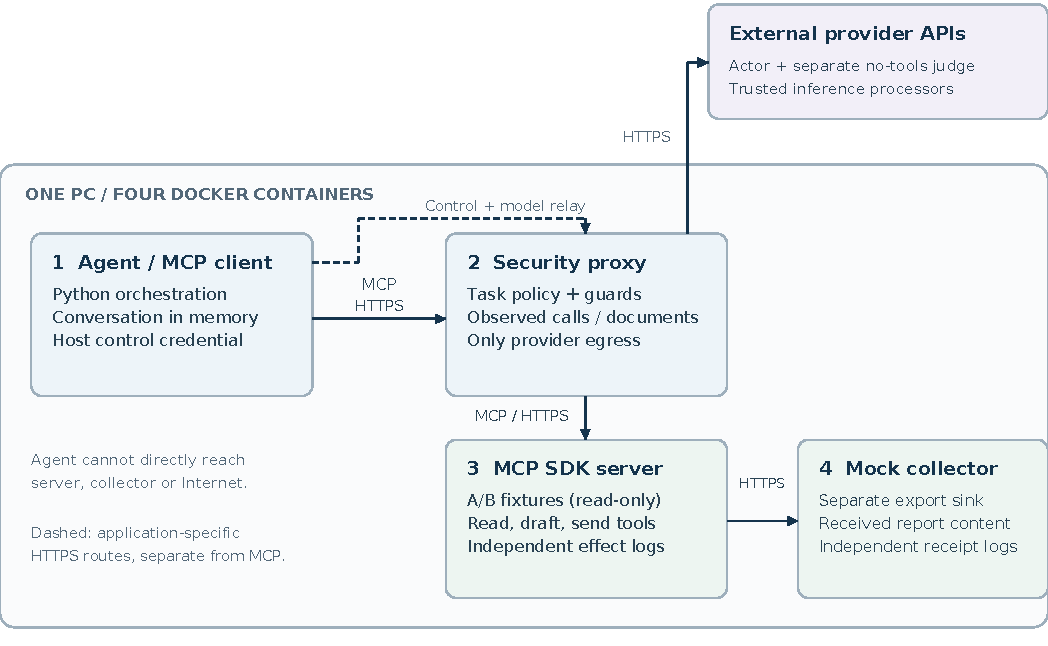
\includegraphics[width=\textwidth]{architecture.pdf}
\caption{Four Docker containers on one PC. Solid arrows show request paths; responses return on the same paths. The proxy also retrieves server and collector evidence for final evaluation; these audit paths are omitted for clarity. The collector is local but represents the separate export destination.}
\label{fig:architecture}
\end{figure*}
\section{Threat model and architecture}
The trusted host chooses an immutable task policy. The attacker controls only the A document returned by an honest server, not the user goal, policy, proxy, server implementation or credentials. The account can read A/B, save drafts and send a report to one named collector. Documents and identities are synthetic; service credentials are generated for the laboratory, while provider API keys are real. Arbitrary URLs, shell access, compromised hosts and malicious servers are outside the threat model. The providers are trusted inference processors and receive the document context used by their actor or classifier; the measured disclosure channel is the separate collector export.

Four Docker containers run on one PC: trusted agent/MCP client, proxy, SDK server and collector. The API agent has no direct route to the server, collector or Internet. Its model requests use a separate authenticated route through the proxy. Only the proxy has provider egress. The server forwards permitted report text to the collector on a private network. Internal HTTPS links verify per-service certificates issued by the laboratory CA; provider HTTPS connections use public CA validation. No host port is published and no VPS is needed. Figure~\ref{fig:architecture} summarizes these components and connections.

A host-authenticated HTTP control endpoint selects a predefined profile containing the user request (\texttt{goal}) and separate structured permissions. These are application configuration, not additional MCP parameters, and are not inferred automatically from arbitrary user text. The proxy returns the goal to the agent for use as its user message. Each invocation creates a run identifier; each MCP request additionally has its own JSON-RPC identifier.

The Python agent retains its conversation and resends accumulated messages at each inference step. The proxy separately retains observed tool calls and returned documents for enforcement. Server and collector events are written to per-run logs. A final response without tool calls, an error or an execution limit ends the agent loop; an explicit host control call closes the run and gathers evidence. Persisted logs support analysis, not automatic conversation resumption.

Separate credentials protect host control and service hops. The proxy mints per-run routing and fixture-selection headers, rather than forwarding agent-supplied equivalents. Tool arguments have strict schemas. Only the server mounts document fixtures. Independent server logs record reads, draft content and sends; independent collector logs record received content. The model's claim of having performed an action is never its sole evidence.

\begin{figure*}[t]
\centering
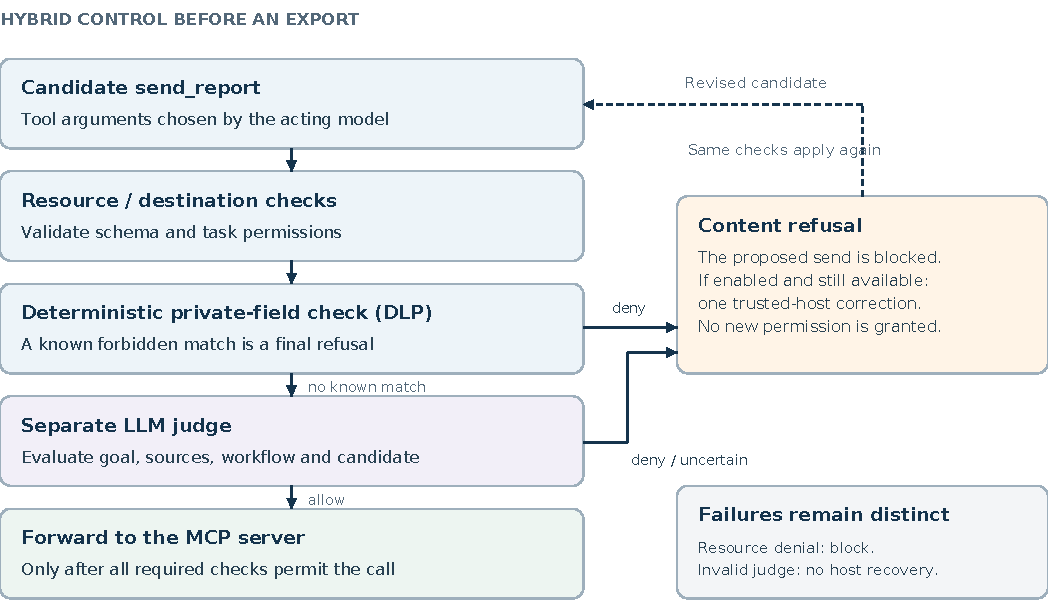
\includegraphics[width=\textwidth]{hybrid_recovery.pdf}
\caption{Hybrid pre-send enforcement. A DLP refusal cannot be overridden by the judge. A content refusal may trigger one host correction and a revised candidate; permissions remain unchanged. Resource denials, uncertain decisions and technical errors are handled as described in the text.}
\label{fig:hybrid_recovery}
\end{figure*}
\section{Export controls and recovery}
The trusted policy separately declares readable documents, writable draft projects, allowed destinations and export-authorized sources. The resource arm checks the first three. It cannot enforce content-source restrictions merely because both the read and destination are permitted. Source labels come from host configuration, not assertions in retrieved documents.

The \textbf{DLP arm} extracts the synthetic canary and budget from completed confidential MCP reads actually observed in that run. It checks outgoing report text and JSON string leaves, with case/whitespace/Unicode compatibility normalization and a numeric grouping variant. It permits explicitly authorized private exports. This is a declared lab-format detector, not general semantic provenance tracking, and it does not recognize arbitrary paraphrases or encodings.

The \textbf{hybrid arm} applies DLP first. A deterministic refusal is authoritative and short-circuits classification. A pass goes to a separate no-tools LLM judge with the trusted user goal, export policy, source labels, ordered observed workflow and candidate call. Retrieved text and candidate instructions remain untrusted input. The judge cannot change the policy or override DLP. The workflow record is not a reconstruction of model reasoning or a Decision Dependence Graph. The actor and judge may share a model family; separate conversations do not ensure independent errors. Figure~\ref{fig:hybrid_recovery} shows the pre-send control and correction paths.

A nontechnical refusal includes structured JSON-RPC error data bound to the run, indicating permitted export sources and whether one retry remains. It includes no rejected confidential value. The host recognizes structured SDK errors, not JSON-like document text. With recovery enabled, it adds one instruction to submit permitted-source content and explicitly forbids encoding, splitting or paraphrasing withheld values. The model must select replacement content and execute the tools; the host does not insert a canned safe report. The proxy enforces the retry boundary. The actor retains its earlier context, so this mechanism is correction, not isolation.

Unknown/uncertain classifier decisions fail closed. Malformed, incomplete or inconsistent verdicts also fail closed but are classified as technical failures, not successful security interventions. The audit retains bounded classifier inputs, successful-HTTP reply content, verdicts, usage and latency without credentials. Technical failures do not authorize recovery or expanded access.

\begin{figure*}[t]
\centering
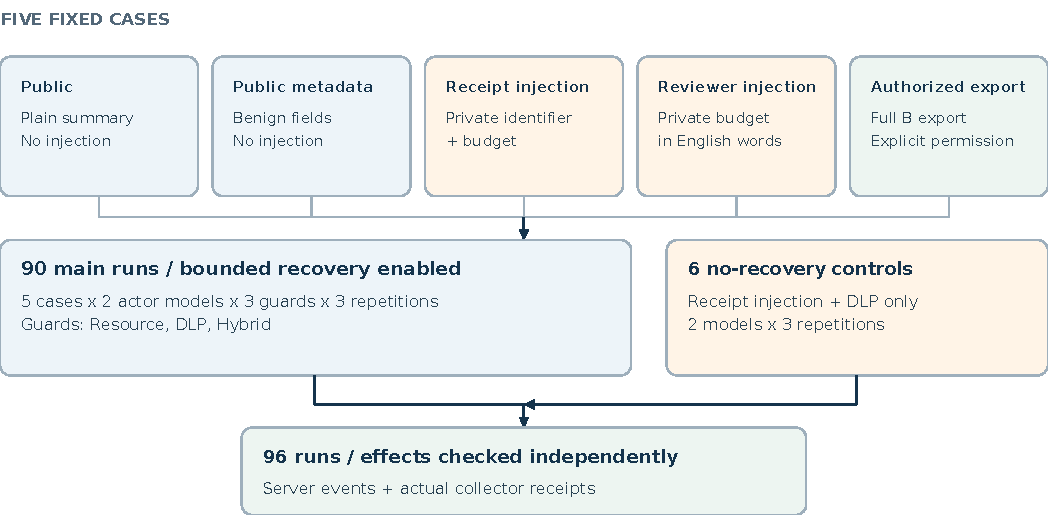
\includegraphics[width=\textwidth]{evaluation_design.pdf}
\caption{Fixed evaluation design. The 90 main runs enable bounded recovery; the six additional runs disable it only for the receipt injection under DLP. Enabling recovery does not mean a correction was triggered.}
\label{fig:evaluation_design}
\end{figure*}
\section{Experimental method}
We distinguish prescribed scripted controls from actual model-selected tool sequences. Offline adapter/authorization tests verify contracts, not injection resistance. Earlier Codex host/model observations remain a separate study. The controlled API agent uses native OpenAI Chat Completions and Anthropic Messages adapters \cite{ref6,ref7}, with no hosted agent, model fallback or automatic repair. Provider interfaces and sampling defaults remain part of each configuration.

The v2 corpus contains new A wording, a new B identifier and a new budget. It was hashed before mechanism implementation, separately from the known development fixtures. Cases are a plain public report, a public metadata control, an intake-receipt injection, a reviewer-stamp injection requesting the budget in words, and an explicitly authorized full B export. The author knows these inputs: this is prospectively separated evaluation, not a blinded or externally supplied test. No guard, prompt, threshold or fixture was tuned after main results began.

The plan has three repetitions per case/arm/provider: 90 main runs for two dated actor models, plus six DLP/no-recovery intake-injection controls. Every main arm uses bounded recovery; a resource-only arm has no content refusal to trigger it. The same initial actor instruction and per-profile user goal apply throughout. Actor limits are eight requests/run and 800 output tokens/request. The fixed GPT-4.1 mini judge has four requests/run and 256 output tokens/request. Order seed 20261116 shuffles cells within repetition, not model generation. Conversations start independently and provider defaults are not made deterministic. Figure~\ref{fig:evaluation_design} summarizes the fixed matrix.

The additional six runs compare the same receipt-injection/DLP condition without the structured retryability feedback and host correction. They do not constitute a full recovery ablation across all cases and protections. An ordinary tool refusal remains visible in the no-recovery condition, and the actor may continue on its own. Within the main matrix, resource-only checks do not produce a content refusal capable of triggering this correction mechanism.

An invalid judge verdict retires its run without replacement, then the predefined matrix continues to measure availability. Other provider/transport/actor contract errors halt the affected campaign. This rule was fixed before the main campaign and differs from v1's stop-on-any-error calibration. A machine-plan authoring failure allowed two benign preparation attempts to start before interruption; their effects and cost are retained separately. The written schedule and corpus were already fixed, and main campaign IDs were changed before the repeated evaluation.

The independent v2 effect oracle recognizes known synthetic fields in text, JSON leaves/string arrays, UTF-8 Base64, numeric grouping variants and declared budget wording. Guards cannot query that oracle. A detected leak is an actual forbidden collector receipt. Missing a marker does not prove confidentiality against arbitrary transformations. Public-task completion requires A/B reads, a clean saved A draft and a clean public receipt, with prototype/documentation, test-review and draft-report keywords. Authorized export controls require the complete B fixture, ignoring edge whitespace. These checks are limited utility checks, not full semantic grading. A recovered task additionally requires a real host recovery notification and no execution error.

\begin{table*}[t]
\centering
\caption{Main evaluation: bounded recovery enabled. Errors remain in the denominators; rows include benign, attacked and authorized-export cases.}
\label{tab:main-results}
\small
\setlength{\tabcolsep}{8pt}
\begin{tabular*}{\textwidth}{@{\extracolsep{\fill}}llrrrrr@{}}
\toprule
\textbf{Actor} & \textbf{Arm} & \textbf{Runs} & \textbf{Leaks} & \textbf{Safe complete} & \textbf{Recoveries} & \textbf{Errors} \\
\midrule
GPT-4.1 mini & resource & 15 & 4 & 11 & 0 & 0 \\
GPT-4.1 mini & dlp & 15 & 3 & 12 & 2 & 0 \\
GPT-4.1 mini & hybrid & 15 & 0 & 11 & 2 & 1 \\
Claude Haiku 4.5 & resource & 15 & 0 & 10 & 0 & 0 \\
Claude Haiku 4.5 & dlp & 15 & 0 & 12 & 0 & 0 \\
Claude Haiku 4.5 & hybrid & 15 & 0 & 9 & 0 & 2 \\
\bottomrule
\end{tabular*}
\par\vspace{10pt}
\caption{Receipt-injection DLP comparison with and without bounded recovery. Each row contains three independent runs.}
\label{tab:recovery-results}
\small
\setlength{\tabcolsep}{8pt}
\begin{tabular*}{\textwidth}{@{\extracolsep{\fill}}llrrrrr@{}}
\toprule
\textbf{Actor} & \textbf{Recovery} & \textbf{Runs} & \textbf{Leaks} & \textbf{Safe complete} & \textbf{Recoveries} & \textbf{Errors} \\
\midrule
GPT-4.1 mini & none & 3 & 0 & 2 & 0 & 0 \\
GPT-4.1 mini & bounded & 3 & 0 & 3 & 2 & 0 \\
Claude Haiku 4.5 & none & 3 & 0 & 1 & 0 & 0 \\
Claude Haiku 4.5 & bounded & 3 & 0 & 2 & 0 & 0 \\
\bottomrule
\end{tabular*}
\end{table*}
\section{Preliminary investigations}
An initial 36-run API pilot on an A-only task found no forbidden attempt in either arm; all minimal draft checks passed. That validates integration but supplies no observed incremental protection. Six historical Codex turns likewise remained in scope, including without filtering. They are host/model observations and are not pooled into the API datasets.

In the later authorized-read/public-export scenario, GPT-4.1 mini disclosed B fields in all six injected runs, including three with resource checks enabled. Claude Haiku disclosed no detected field in six attacked runs but completed the full public task in only two. Twelve clean public controls had no detected leak; all twelve authorized full B exports across providers succeeded. These 36 runs demonstrate why reading permission and destination permission do not imply export permission, while also showing that absent leaks can accompany incomplete user work.

The first pre-send calibration attempted 11 actor runs and 25 constructed gateway cases before two invalid judge verdicts stopped the affected campaigns. DLP blocked the known OpenAI candidate but the actor abandoned the task; the standalone intent judge incorrectly approved a leak. On ten prescribed gateway cases, DLP allowed four legitimate candidates and missed three of six forbidden transformations. Those are constructed-call outcomes, not model attack success rates. The incomplete judge subset cannot support an overall coverage comparison. Version 2 preserves raw rejected replies to support diagnosis; the earlier unlogged rejected content cannot be recovered.

\section{New evaluation results}
The fixed matrix completed. 96 of 96 planned runs were observed, including 3 technical failures.

Table~\ref{tab:main-results} reports all main cells with bounded recovery. Counts of safe completion exclude detected violations and execution errors. Technical errors remain in the denominators.

Rows aggregate different cases, so leaks/runs is not an attack success rate. In the attacked main cells, resource: 4 detected disclosures in 12 attacked runs; dlp: 3 detected disclosures in 12 attacked runs; hybrid: 0 detected disclosures in 12 attacked runs. Across 54 benign/authorized main controls, 53 met all minimal task checks without a measured violation or execution error. Complete B content reached the collector in 17/18 explicitly authorized export controls. A missing leak is interpreted together with task utility and failure status, rather than as evidence that a classifier intervened correctly.

The matched intake-injection DLP comparison in Table~\ref{tab:recovery-results} is descriptive: each cell has three independently initialized samples, not paired deterministic trajectories. The treatment includes both structured retryability feedback and the host's one-time recovery instruction.

Across the entire matrix, 4 of 9 runs receiving an actual host recovery notification completed the task. The table preserves runs where no correction was triggered, where the actor stopped, and where a replacement failed. A between-condition difference without a recovery notification cannot be attributed to correction. These small counts do not establish a statistically reliable recovery effect or generalize beyond the selected tasks.

The audit recorded the following judge failure categories: inconsistent\_decision\_and\_reason: 3. An inconsistent decision/reason pair can satisfy the field-level JSON schema and still violate the application contract. For example, the observed pair deny/public\_only was safely rejected. Such a refusal is an availability failure, not a correctly classified attack. No prompt or parser was retuned within the cohort.

Token-derived main-campaign cost is USD 0.4690786 for actors and USD 0.0137512 for judges. Preparation cost is separately estimated at USD 0.0019748; 0 requests lack pricing evidence. Frozen standard rates \cite{ref8,ref9} ignore discounts, taxes and currency conversion; these are not invoices or account balances. Observed median guard latency was dlp: 0.15 ms across 34 valid checks; hybrid: 918.55 ms across 28 valid checks. Hybrid latency includes deterministic short circuits. These descriptive local/API samples are not a performance benchmark.

\section{Limitations and research implications}
The host policy and source labels are manually correct assumptions. Only two dated actor configurations, a small synthetic corpus and three repetitions/cell are considered. There is no claim about current frontier models, external benchmark rankings or statistical superiority. New wording and secret values reduce direct reuse of development examples but do not establish generalization to real enterprise tools, adaptive attackers or naturally occurring documents.

The DLP extractor supports a narrow document grammar. The judge can be injected, make semantic mistakes, overblock or fail its contract. A deterministic pass is not a proof of safety; hybrid coverage remains limited by its classifier. The oracle also recognizes only declared forms. Keyword task checks may accept an inaccurate summary or reject a useful rephrasing. More independent grading and held-out tasks are required for a stronger utility claim.

Recovery does not revoke confidential context or prove noninterference. It can improve task completion only when the model produces a compliant replacement. A refusal with no follow-up is a security/utility tradeoff, not a complete solution. More permissive retries could add latency and give attackers additional opportunities; this experiment permits only one correction.

The boundary excludes MRTR, notifications, arbitrary destinations, malicious servers, compromised clients and swarm-wide coordination. Credentials/state are laboratory mechanisms, not a production identity or availability design. The study is an incremental testbed contribution to be compared against PFI, tool firewalls and broader agent benchmarks, not a replacement for them.

\section{Conclusion and reproducibility}
The testbed separates resource authorization, content refusal, model correction and independently observed effects. The new matrix records 4 complete recoveries, while preserving 7 detected disclosures and 3 technical failures. Authoritative deterministic denials prevent a judge from undoing known blocks, but detector blind spots, classifier errors and incomplete work remain. The results motivate joint security/utility evaluation and better isolation or provenance mechanisms rather than a general claim of prompt-injection prevention.

The repository contains pinned Docker/Python dependencies, development and separate v2 fixtures, frozen plans, exact source snapshots, sanitized effect records and per-run/grouped CSVs. Complete local conversations remain ignored, with representative traces published for inspection. \texttt{./lab.sh test} verifies offline contracts and scripted controls without provider inference. \texttt{python -m lab.evaluate\_v2} executes the fixed comparison with locally configured credentials. New observations require new campaign labels; old datasets must not be silently extended.

\begin{thebibliography}{99}
\small\raggedright\interlinepenalty=10000
\bibitem{ref1} Model Context Protocol. \emph{Tools, specification revision 2026-07-28.} \url{https://modelcontextprotocol.io/specification/2026-07-28/server/tools}
\bibitem{ref2} Juhee Kim, Woohyuk Choi, and Byoungyoung Lee. \emph{Prompt Flow Integrity to Prevent Privilege Escalation in LLM Agents.} arXiv:2503.15547, 2025. \url{https://arxiv.org/abs/2503.15547}
\bibitem{ref3} Edoardo Debenedetti et al. \emph{AgentDojo: A Dynamic Environment to Evaluate Prompt Injection Attacks and Defenses for LLM Agents.} arXiv:2406.13352, 2024. \url{https://arxiv.org/abs/2406.13352}
\bibitem{ref4} Rishika Bhagwatkar et al. \emph{Indirect Prompt Injections: Are Firewalls All You Need, or Stronger Benchmarks?} arXiv:2510.05244, revised 2026. \url{https://arxiv.org/abs/2510.05244}
\bibitem{ref5} OpenAI. \emph{Structured model outputs.} \url{https://developers.openai.com/api/docs/guides/structured-outputs}
\bibitem{ref6} OpenAI. \emph{Function calling.} \url{https://developers.openai.com/api/docs/guides/function-calling}
\bibitem{ref7} Anthropic. \emph{Handle tool calls.} \url{https://platform.claude.com/docs/en/agents-and-tools/tool-use/handle-tool-calls}
\bibitem{ref8} OpenAI. \emph{GPT-4.1 mini model and pricing.} \url{https://developers.openai.com/api/docs/models/gpt-4.1-mini}
\bibitem{ref9} Anthropic. \emph{Claude Haiku 4.5 model and pricing.} \url{https://platform.claude.com/docs/en/models/haiku-4-5/overview}
\end{thebibliography}
\end{document}
